\newpage
\appendix


%%%%%%%%%%%%%%%%%%%%%%%%%%%%%%%%%%%%%%%%%%%%%%%%%%%%%%%%%%%%%%%%%%%%%%
%%%%%%%%%%%%%%%% Deep Learning with label noise       %%%%%%%%%%%%%%%%
%%%%%%%%%%%%%%%%%%%%%%%%%%%%%%%%%%%%%%%%%%%%%%%%%%%%%%%%%%%%%%%%%%%%%%

\section{Convolutional Networks for Semantic Segmentation}

\noindent
The different levels of hierarchical features in CNNs are believed to play different roles in extracting information from the images.
The low-level features process the local information within small neighborhood and the high-level features ensemble information from lower-level features to extract abstract information.
The high-level features were found to significantly dependent on the exact categories compared to the low-level features which show extraordinary category independence.\cite{yosinski2014transferable}
Previous studies\cite{sukhbaatar2014training,patrini2016making} have shown that training with noisy labels can lead to significantly higher classification errors than training with clean labels if the total number of training samples are fixed.
It is nevertheless unclear how the annotation errors would influence the learned multiple level features.
We made a hypothesis that annotation errors do not necessarily lead to a ``bad representation'' because the ``generality'' of low-level features may contribute to a robustness to the errors when we transfer the learned features to a new dataset with new categories.
\footnote{M: We hypothesize?
For the rest I find the actual hypothesis pretty vague.  Firstly, you use quotation marks quite often, which doesn't make ``things'' clearer.  Either don't use that and make sure that the words you use are indeed the words you like to say or expand the part between ``''s and use some more sentences to really explain what you have in  mind.  Secondly, for me the part ``contribute to a robustness to the errors'' needs further explaining.  You might not have to get mathematically precise here, but I don't understand what you want to say here...}

\noindent \textit{Narrow the problem of discussion down to Segmentation}
The state-of-art DCNN based semantic image segmentation models relies on transferring the pre-trained convolutional filters as well.\cite{long2015fully}
A typical method to pre-train the convolutional filters is to train a classification model with the large-scale ILSVRC dataset \cite{russakovsky2015imagenet}
However, this method constrains the semantic image segmentation models to have the same CNN architecture as the image classification models.
The CNN design for semantic image segmentation does not necessarily follow the design of image classification architectures.
The segmentation models need both global and local information to predict the category and give a fine segmentation, whereas the classification models care less about local information for object localization.
For instance, the presence of the max-pooling layers enable the following convolutional filters to have larger receptive fields but, at the same time, reduce the resolution of the features.
\footnote{M: Is it the presence of max-pooling or the presence of subsampling that enables larger receptive fields?  And what do you mean by resolution?  Should low resolution always mean reduced / ``thrown away'' information? J: Max-pooling is a particular type of subsumpling. Actually both the conv layers and the pooling layers lead to gradually larger receptive field.}
Additional upsampling layers can recover the shape of the output segmentation but cannot fully recover the information dropped by subsampling.
This first-pooling-and-then-upsampling pipeline can result in coarse segmentation output \cite{chen2016deeplab} with non-shape boundaries and blob-like shapes.
\footnote{M: Also for this claim, I think we need a reference or something like that. Or other proof indeed...  In addition, I wonder whether we can explain why this may be the case? J: Yes, I can refer to a paragraph in the intro of CRFasRNN and enrich the discussion a bit.}
%The coarse output can be refined with Conditional Random Field (CRF) inference\cite{zheng2015conditional,chen2016deeplab}.
\noindent
Alternatively, one can also extract convolutional features with semantic segmentation tasks.
But it is more difficult to collect well-annotated dataset for semantic image segmentation than for object recognition.
A large number of annotated images are of great value to train sufficiently generalized representation and avoid overfitting, given the ``data-hungry'' nature of DCNNs.
\footnote{M: For the rest a bit vague... what do we really mean by suffer? Maybe this becomes clear later in the intro...? J: Refrased. M: This is still quite unclear to me.  I would interpret ``data-hungry'' as an NN that overtrains even with large amount of data, but one would typically try to fix this by introducing some form of regularization or just using smaller networks.  All in all [as a maybe-too-stubborn non-deep learner  ;-)  ] I could still wonder what is really the problem...}
Allowing noisy annotations to exist could help significantly increase the number of annotated images and the number of training samples could compensate the impact of annotation errors.
We will further discuss this in the related works.


%%%%%%%%%%%%%%%%%%%%%%%%%%%%%%%%%%%%%%%%%%%%%%%%%%%%%%%%%%%%%%%%%%%%%%
%%%%%%%%%%%%%%%% Deep Learning with label noise       %%%%%%%%%%%%%%%%
%%%%%%%%%%%%%%%%%%%%%%%%%%%%%%%%%%%%%%%%%%%%%%%%%%%%%%%%%%%%%%%%%%%%%%

\section{Deep Learning with Label Noise}

\section{}



%%%%%%%%%%%%%%%%%%%%%%%%%%%%%%%%%%%%%%%%%%%%%%%%%%%%%%%%%%%%%%%%%%%%%%
%%%%%%%%%%%%%%%% Appendix Results                     %%%%%%%%%%%%%%%%
%%%%%%%%%%%%%%%%%%%%%%%%%%%%%%%%%%%%%%%%%%%%%%%%%%%%%%%%%%%%%%%%%%%%%%

%%%%%%%% FIGURE Number of training categories
\begin{figure}[t]
\centering
   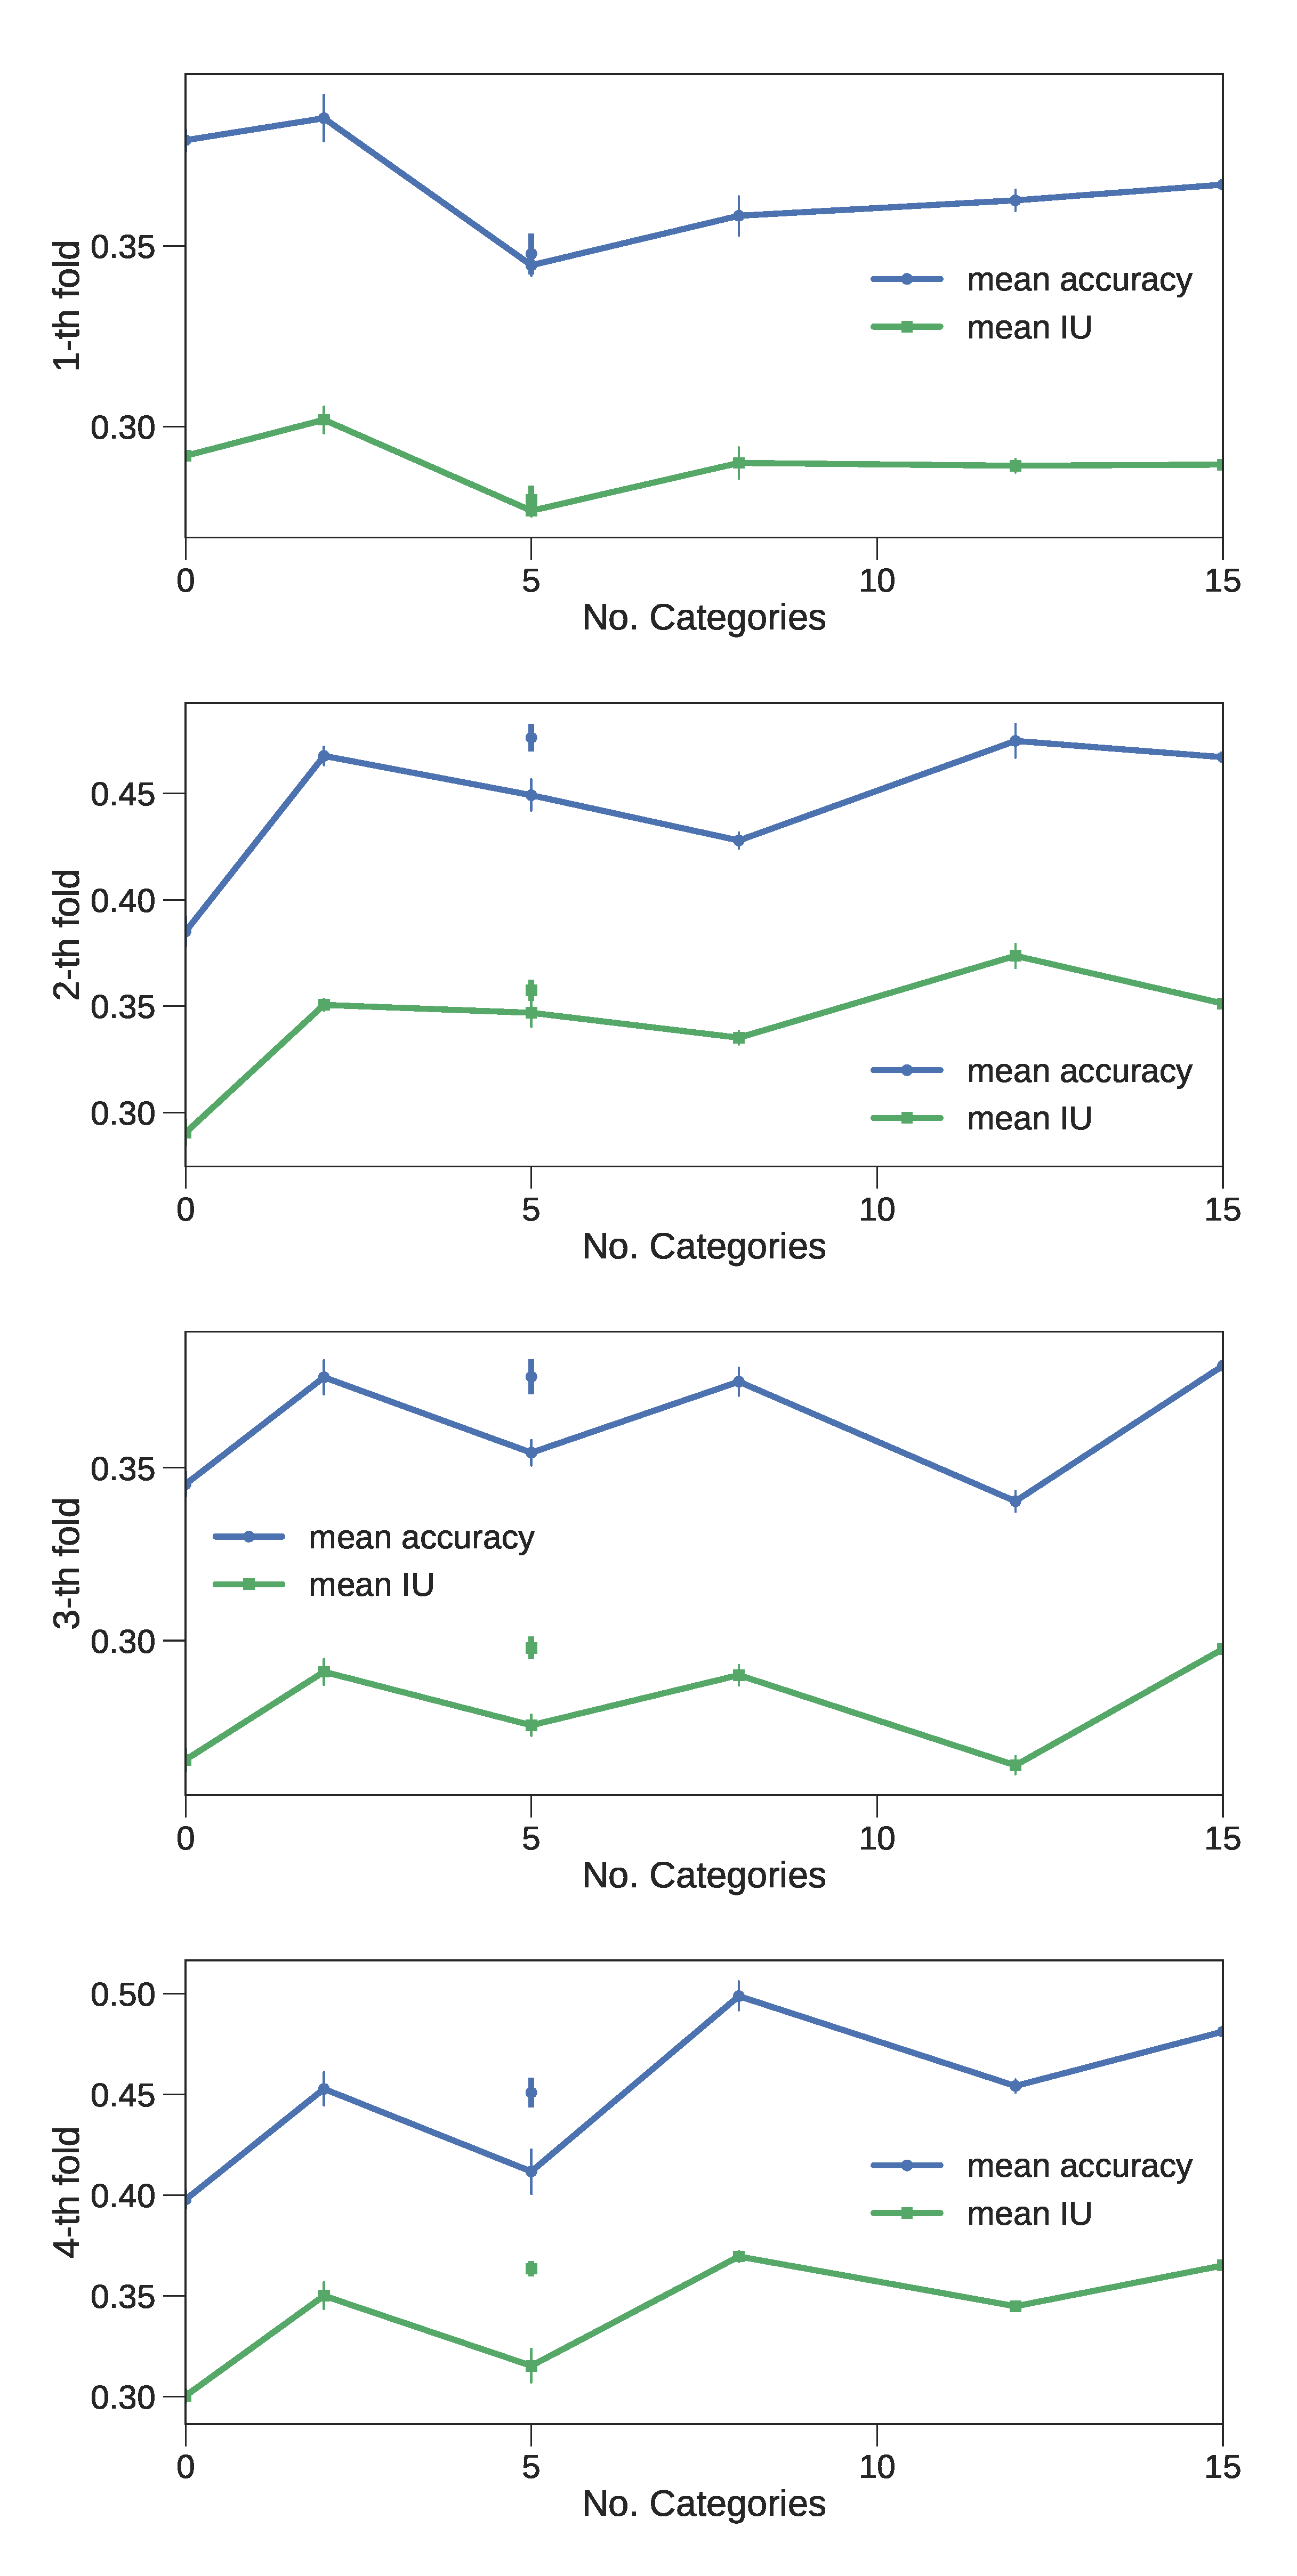
\includegraphics[width=\linewidth]{img/num_classes_folds.eps}
\caption{The influence of number of pre-training categories on performance of fine-tuned models for each fold, addition to Figure \ref{fig:categories}.}
\label{fig:classesfold}
\end{figure}
